%\documentclass[11pt,a4paper]{article}
%\usepackage[hyperref]{emnlp2021}
%\usepackage{times}
%\usepackage{latexsym}
%\usepackage{graphicx}
%\usepackage{natbib}
%\usepackage{amsmath}
%\usepackage{amsfonts}
%\usepackage{url}
%\usepackage{multirow}
%\usepackage{booktabs}
%\usepackage{bm}
%\usepackage[linesnumbered, boxed, ruled]{algorithm2e}
%
%\renewcommand\arraystretch{1.2}
%\setlength\parskip{0.1\baselineskip}
%\setlength{\textfloatsep}{0.5cm}
%% This is not strictly necessary, and may be commented out,
%% but it will improve the layout of the manuscript,
%% and will typically save some space.
%\usepackage{microtype}
%\newcommand{\secref}[1]{Section \ref{#1}}
%\newcommand{\figref}[1]{Figure \ref{#1}}
%\newcommand{\eqnref}[1]{Eq. (\ref{#1})}
%\newcommand{\tabref}[1]{Table \ref{#1}}
%\usepackage[hyperref]{emnlp2021}
%\usepackage{times}
%\usepackage{latexsym}
%\usepackage{graphicx}
%\usepackage{natbib}
%\usepackage{amsmath}
%\usepackage{amsfonts}
%\usepackage{url}
%\usepackage{multirow}
%\usepackage{booktabs}
%\usepackage{bm}
%\usepackage[linesnumbered, boxed, ruled]{algorithm2e}
%\usepackage{tikz}
%\usepackage{geometry}
%%\usetikzlibrary{automata,positioning}
%%\geometry{left=2.0cm, right=2.0cm, top=2.5cm, bottom=2.5cm}
\documentclass[letterpaper]{article}
\usepackage{aaai22}  % DO NOT CHANGE THIS                                                                              
\usepackage{times}  % DO NOT CHANGE THIS
\usepackage{helvet}  % DO NOT CHANGE THIS
\usepackage{courier}  % DO NOT CHANGE THIS
\usepackage[hyphens]{url}  % DO NOT CHANGE THIS
\usepackage{graphicx} % DO NOT CHANGE THIS
\urlstyle{rm} % DO NOT CHANGE THIS
\def\UrlFont{\rm}  % DO NOT CHANGE THIS
\usepackage{natbib}  % DO NOT CHANGE THIS AND DO NOT ADD ANY OPTIONS TO IT
\usepackage{caption} % DO NOT CHANGE THIS AND DO NOT ADD ANY OPTIONS TO IT
\DeclareCaptionStyle{ruled}{labelfont=normalfont,labelsep=colon,strut=off} % DO NOT CHANGE THIS
\frenchspacing  % DO NOT CHANGE THIS
\setlength{\pdfpagewidth}{8.5in}  % DO NOT CHANGE THIS
\setlength{\pdfpageheight}{11in}  % DO NOT CHANGE THIS
%\usepackage{algorithm}
%\usepackage{algorithmic}

\usepackage{newfloat}
\usepackage{listings}
\lstset{%
    basicstyle={\footnotesize\ttfamily},% footnotesize acceptable for monospace
    numbers=left,numberstyle=\footnotesize,xleftmargin=2em,% show line numbers, remove this entire line if you don't want the numbers.
    aboveskip=0pt,belowskip=0pt,
    showstringspaces=false,tabsize=2,breaklines=true}

\usepackage{microtype}
\usepackage{natbib}
\usepackage{caption}
\usepackage{helvet}
\usepackage{amsmath}
\usepackage{amsfonts}
\usepackage{tikz}
\usepackage{graphicx}
\usepackage{multirow}
%\usepackage[usenames,dvipsnames]{color}
%\usepackage{color, colortbl}
%\usepackage{subfigure}
\usepackage{url}
\usepackage{bm}
\usepackage{booktabs}
\usepackage{verbatim}
\usepackage[noend]{algpseudocode}
\usepackage{algorithmicx,algorithm}
\usepackage{bbding}
\usepackage{subcaption} 
%\setcounter{secnumdepth}{2} %May be changed to 1 or 2 if section numbers are desired.
%\usepackage{aaai22}
%\usepackage{times}
%\usepackage{latexsym}
%\usepackage{graphicx}
%\usepackage{natbib}
%\usepackage{amsmath}
%\usepackage{amsfonts}
%\usepackage{url}
%\usepackage{multirow}
%\usepackage{booktabs}
%\usepackage{bm}
%\usepackage[linesnumbered, boxed, ruled]{algorithm2e}
%\usepackage{bbding}
\newcommand{\crosssymbol}{{ \XSolidBrush} }
%{{\color{red} \XSolidBrush} }
\newcommand{\checksymbol}{{\Checkmark} }
%\renewcommand\arraystretch{1.2}
%\setlength\parskip{0.1\baselineskip}
%\setlength{\textfloatsep}{0.5cm}
% This is not strictly necessary, and may be commented out,
% but it will improve the layout of the manuscript,
% and will typically save some space.
\newtheorem{example}{Example}
\usepackage{microtype}
\newcommand{\secref}[1]{Section \ref{#1}}
\newcommand{\figref}[1]{Figure \ref{#1}}
\newcommand{\eqnref}[1]{Eq. (\ref{#1})}
\newcommand{\tabref}[1]{Table \ref{#1}}
\newcommand{\exref}[1]{Example \ref{#1}}
\newcommand{\cut}[1]{}
%\usepackage{float}
%\usepackage{tikz}
%\usepackage{subfigure}
%\usepackage{graphicx}
%\setlength\footskip{0pt}
%\setlength\headsep{0pt}
%\setlength\topmargin{-50pt}
%\setlength\textheight{800pt}
\title{xxxx}
\author{}
\date{}
\begin{document}

\subsection{Reviewer \#1}
\textbf{Q1: Can you tell me whether this idea has been...}

\noindent
\textbf{A1:} Even though our mutation operator is operationally similar to the random token 
swapping (RS) operator in previous work
%lots of work mentioned randomly swapping tokens (mutation)
(Artetxe et al., 2018; Lample et al., 2018; Wei and Zou, 2019; Miao et al., 2020), 
the purpose is different.
The purpose of RS is to improve models' fault tolerance by perturbing 
the sentence without changing its meaning; 
the purpose of our mutation is to encourage the models to look into the 
premise (avoid short-circuits). 
Consequently, the way we construct the data is also different which is 
illustrated in the following figure. 
\begin{figure}[th]
 	\centering
 	\includegraphics[width=0.9\columnwidth]{figure/revised_mutation.eps}
 	%\caption{Mutation operation
    %    swaps two consecutive words either in the right choice
    %    or wrong choice of the original MCQ.}
 	\label{fig:mutation}
\end{figure}
We will update Fig 3 in the paper with this figure. 

%falsify the sentence, i.e., after mutation, the 
%right choice sentence becomes wrong and the wrong choice stays wrong. We can modify Figure 3 
%to 
%'t change the semantic of natural language. 
%After mutation operation, the right choice is still right and wrong choice is still wrong. 
%is sensitive to text order information, while slight order change is still readable for humans. 
%Therefore, the mutation 
%within a reasonable range can be used as a data augmentation method. 
%However in our method, we treat the choices with mutation operation on right as 
%a wrong choice which is more strict than previous work. 
%We show mutation operator thoroughly in \figref{fig:mutation}. 
%In augmented samples, the right choice will be preserved. 
%The wrong choice can be derived from original right choice (yellow) or wrong choice (pink). 
%We will randomly choose one from A1 and A2 as a new sample.
%We mutate on the right choice (yellow) in A1 to be wrong because we want 
%to encourage the
%model to look into the premise due to its two very similar
%choices (same set of tokens).
%Besides, it can also make the model more
%sensitive to find differences in word orders and enhances the
%model’s prior grammatical knowledge (described in Sec 2.3). 
%%We also mutate on wrong choice to be wrong, because we expect to break some bias feature in 
%%wrong choice. 

%We ensure the correctness of augmented data with this strict operation. 
%We sampled 100 samples from the mutated 
%samples and annotated these samples by 5 annotators on ROC. The accuracy for these 
%questions is always 100%. You may also wonder to know which kind of mutation is better. 
%If we believe mutation keeps its meaning and augment data with this operator, 
%although it can enhance fault tolerance of models, it does nothing for bias  
%elimination which is the main reason for model fragility in MCQ tasks. Because the 
%feature distribution based on different label is almost unchanged as the meaning.


\noindent
\textbf{Q2: Can you extend this idea to more settings...}

\noindent
\textbf{A2:} Good suggestion. One of our 4 datasets, RECLOR, is already 
an MRC dataset. We can include more in the final version. 
%We have utilized 4 datasets on different tasks 
%to show the effectiveness of our methods including RECLOR which is a widely used 
%multiple choice machine reading comprehension dataset. We can extend to more datasets 
%in appendix in our revised version. 

\subsection{Reviewer \#2} 

Thank you very much for your good suggestions.

\noindent
\textbf{Q1: Mutation in Fig 3 unclear...} 

\noindent
\textbf{A1:} Please refer to A1 of Reviewer \#1 and the beginning of Sec 2.2 for the motivation of 
the two operators.

%Our description maybe not clear enough that make you confused 
%on 
%In fact, we always preserve the right choice. For the generated wrong choices, 
%they can be derived from the right choices or wrong choices. For example, In Figure3, The 
%right choice can be denoted as R, the wrong choice with color pink can be denoted as W. 
%Then the swapped sentence from R and W are R' and W'. R' and W' are both wrong choices because 
%they are grammatically wrong. Then we can randomly choose R' or W' as a wrong choice for the 
%new aumgmented question A'.

\noindent
\textbf{Q2: the dataset size is relatively small...}

\noindent
\textbf{A2:} Please refer to A7 of Reviewer \#3.

\subsection{Reviewer \#3}

\noindent
\textbf{Q1: In Figure 1, is there an impact...}

%\textbf{A1:} Figure 1, \figref{fig:mlm}, and \figref{fig:cross_mlm} 
\noindent
\textbf{A1:} We followed your advice and compare the attention maps of BERT 
fine-tuned on unlabeled and labeled data in the following figure. 
Despite some very light color in the premise of Fig (a), BERT+C still
shows more obvious effects of ``forcing the model to look at premises''. 
%It also indicates that supervised learning on MCQ tasks can misleading language models.
%\figref{fig:mlm} shows the attention map 

\begin{figure}[th]
\centering
\begin{subfigure}[b]{0.20\textwidth}
\centering
\framebox{\includegraphics[width=\columnwidth]{figure/mlm.eps}}
\caption{BERT fine-tuned on unlabeled COPA}
\label{fig:mlm}
\end{subfigure}
\hfill
\begin{subfigure}[b]{0.20\textwidth}
\centering
\framebox{\includegraphics[width=\columnwidth]{figure/cross_mlm.eps}}
\caption{BERT+C fine-tuned on labeled COPA}
\label{fig:cross_mlm}
\end{subfigure}
%\caption{Attention map on a COPA example for models.}
%\KZ{Caption is wrong! most graphs are fine. 
%But ReCLOR (RB) is a bit strange. 
%Why is BT line exactly the same as the BT+C? And why is BT+B so bad?}}
%\label{fig:case}
\end{figure}


%model without fine-tuning and Figure 1 in \figref{fig:case} 
%(a and b seperately). The result shows that unsupervised learning 

\noindent
\textbf{Q2: questions and answers are rather single...}

\noindent
\textbf{A2:} Thank you for your good suggestion. What you are 
suggesting is hierachical representation scheme which is reasonable but 
uncommon for MCQ type of NL reasoning tasks that this paper is targeting. 
Moreover, of the four datasets, only two (COPA and ARCT) are single-sentence questions. 
Hence we chose to experiment on the three more popular encoders in this area.
%Not all tasks contains single questions and single answers, 
%like ROC which contains 4 sentences in questions, 
%and RECLOR have a long premise which is a reading comprehension task. 
%Although 
%We mainly experiment on three very popular encoders which is also efficient for 
%sovling these reasoning tasks. 
%Besides, Single-sentences encoders 
%have not been used on these reasoning tasks as far as we know. 
We will consider such hierarchical models in our future work.

\noindent
\textbf{Q3: In table 1, about the adverb operator...}

\noindent
\textbf{A3:} We manually selected adverbs (``in fact'', ``actually'', 
``indeed'') as the prefix to the wrong choices. 
The adverb operator is not used for training but for testing. 
The purpose of the adv operator is to trick the models into selecting the wrong choices 
without looking at the premises.
%The size of pool doesn't influence the parameters of models. 
%The size of the pool is 3 which is selected by 
%human from nearly 100 adverbs which can already show the fragility of models. 

\noindent
\textbf{Q4: This may be popular in MCQ papers...}

\noindent
\textbf{A4:} To fine-tune the language models for an MCQ task, we feed LM's final hidden 
vector to a fully connected layer to compute the probability of the right choice. 
We will add this bit to the final version.

%We did miss the description about the strcuture we used to predict the correct answer. 
%``During fine-tuning on a specific MCQ task with language model encoders, like BERT, the final
%hidden vector corresponding to the first input token is used as the aggregate representation
%followed by an extra fully connected layer to compute the probability score of being the right answer.'' 
%We will add this description in Sec 3.1 in the revised version.

\noindent
\textbf{Q5: In C+M data augmentation scheme...}

\noindent
\textbf{A5:} We noted in Sec 3.1 that ``The expanded
data volume is equal to the original data volume and
the size of new train dataset has doubled.'' 
Therefore, training data augmented with +B, +C, +M and +C+M are 
all the same size. In +C+M, the extra data by +C and +M are equal in size.
%It may be not conspicuous or clear enough. In C+M, 
%the total amount of generated data are the same 
%with other augmented data, 
%but each method (C and M) accounts for a half.
%data volume for C accounts for half of original volume and M is also a half. 
%Thus C+M have the same volume with back-translation, C or M alone which is fair for comparing.
%For the results of double augmented data, we conduct experiments on the ROC data set and find that our 
%conclusion is still valid. The original accuracy for B, C, M, and C+M (double volume) are 
%87.07, 86.75, 86.26, 87.02 and stress test accuracy are 83.11, 84.3, 85.79, 86.06.

\noindent
\textbf{Q6: In Table 4, the average of the 4 datasets...}

\noindent
\textbf{A6:} The purpose of the last two columns is to evaluate the 
average performance of each model over four different datasets which are equally important for us. 
%We should weight on the importance rather than confidence.
Just because a dataset has more 
test cases doesn't mean that this task is more important than the others. 
Therefore it is our opinion to not 
use a weighted average score 
which is also echoed by other researchers (Liu et al. 2019b; Devlin et al. 2019; Yang et al. 2019).
%necessary to use a weighted average score on test data volume. 
%Therefore, the importance of these four datasets are equally. 
%And these four datasets are equally important. 
Moreover, these datasets all have a sufficient number of test cases to be statistically significant. 
%Many papers also compare with the average score
%in this way on GLUE tasks 

\noindent
\textbf{Q7: The baseline seems stronger...}

\noindent
\textbf{A7:} We agree with your observations. 
You may also notice that in Table 4, there is a wider accuracy gap on the vanilla (w/o) models
between original test and 
stress test for RECLOR than other datasets, which indicates that RECLOR has more bias and is 
more susceptible to short-circuit. 
%Our methods on RECLOR seems weaker on original test cases compared with vanilla model 
%and back-transltaion. Because there are 
%a large number of bias features in the RECLOR data set which leading to 
%overestimated result. In Table 4, the accuracy gap between 
%the original test and the stress test on models can reach to about 19% on RECLOR, 
%which is much higher than on other datasets. 
%It indicates that models have captured more bias information on RECLOR. 
Therefore, the final test results of the vanilla models on the original test data are less reliable. 
Though our methods slightly underperform the vanilla and +B models in some cases, 
they have a huge advantage over the vanilla and +B on the stress tests and 
subtantially reduced the accuracy gap.

\noindent
\textbf{Q8: In the introduction, the paragraph starting...}

\noindent
\textbf{A8:} We will revise it to ``In contrast, our proposed ...''

%\textbf{Q9: Please double check the list of references.}
%A9: Thanks for your suggestion.

\subsection{Reviewer \#4}
Thank you for your comments. 
Unfortunately, there are some misunderstandings in your comments.
%It's a pity that you may not understand our work according to the description you make 
%in summary part. 
First, this work targets a wide range of MCQ type tasks in NL reasoning, not just NLI. 
%the tasks we experimented on are all MCQs in natural language reasoning area 
%rather than NlI tasks. 
Second, ``crossover'' and ``mutation'' are novel operations we proposed (see A1 of Reviewer \#1). 
Whereas ``back-translation'' is a strong baseline we compare with.
%the methods we proposed and 
%``back-translation'' is the strong baseline we compared with. We didn't only ``adopt'' them. 
%Third, our experiments show our proposed methods can improve the robustness of vanilla models and 
%they are better than back-translation, a well-know data augmentation method. 
Besides, we also did a detailed analysis in Sec 3.2-3.4.
%the reason for this improvement with detailed
%stress test, choice-only test and case study. We conclude that
%our data augmentation methods can encourge models to pay
%more attention to the premise of questions.
%Thus, we implore you to read our paper carefully again and thanks a lot.

\end{document}
